\section{Introduction to System Design}
System Design translates the abstract logical requirements into a concrete blueprint detailing how the software components will interact, how data will flow through the mathematical pipelines, and how the user interfaces will trigger underlying backend inferences. For CyberShield, the architecture is designed as a modular intelligence platform, encapsulating data processing, machine learning inference, Human-in-the-Loop (HITL) queuing, and PDF generation within a unified operational context.

\section{System Architecture Concept}
The overall architecture follows a Model-View-Controller (MVC) paradigm, distinctively augmented by an offline Machine Learning (ML) pipeline loop. The backend operates as a modular monolith. The ML pickle files act as a completely separate service layer distinct from the traditional database Model layer, ensuring that model inference logic remains decoupled from standard data retrieval.

\begin{itemize}
    \item \textbf{The View (Presentation Layer):} Hosted via Flask templates, this layer provides two drastically different interfaces based on OAuth scopes. The citizen view focuses on minimalistic text input and PDF output. The admin view provides rich dashboard metrics, pending label queues, and retraining controls.
    \item \textbf{The Controller (Routing \& Logic):} The Flask \texttt{app.py} file dictates business logic. It handles the RESTful routes, manages active user sessions via secure cookies, processes Form Data, and invokes the computational sub-modules (prediction, velocity logging, PDF generation).
    \item \textbf{The Model (Intelligence Layer):} Contains two facets: the SQLite database (\texttt{cybershield.db}) which holds stateless records of complaints and artifacts, and the Pickled Serialization space (\texttt{final\_vectorizer.pkl}, \texttt{final\_models.pkl}) which loads the active RAM state of the mathematical ensemble.
    \item \textbf{The Retrain Pipeline (Asynchronous Daemon):} An isolated subsystem (\texttt{pipefinal.py}) that operates entirely offline. It connects to the database, extracts new truths, recalculates TF-IDF boundaries, identifies hard negatives, cross-validates, and writes new models to disk without blocking the main Web Server.
\end{itemize}

\begin{figure}[H]
    \centering
    \resizebox{\textwidth}{!}{%
    \begin{tikzpicture}[
        node distance=0.6cm,
        layer/.style={
            rectangle, draw=black, thick, text=black,
            text width=0.85\textwidth, align=center, rounded corners,
            minimum height=1.5cm, inner sep=8pt
        },
        arrow/.style={thick, ->, >=stealth, draw=black}
    ]
    
    \node[layer, fill=blue!18] (view) {\textbf{Layer 1 --- Presentation Layer (The View)}\\Hosts Citizen and Admin interfaces via Flask templates. Manages raw text input, NCRP PDF output, and OAuth-gated dashboard metrics.};
    
    \node[layer, fill=teal!18, below=of view] (controller) {\textbf{Layer 2 --- Routing \& Logic Layer (The Controller)}\\The Flask \texttt{app.py} engine controls business logic. It handles RESTful API routes, manages secure user sessions, and invokes computational sub-modules.};
    
    \node[layer, fill=orange!22, below=of controller] (model) {\textbf{Layer 3 --- Intelligence Layer (The Model)}\\SQLite (\texttt{cybershield.db}) stores historic stateless complaints. Serialized ML pickles provide high-speed inference scoring in RAM.};
    
    \node[layer, fill=violet!18, below=of model] (retrain) {\textbf{Layer 4 --- Retrain Pipeline Layer (Asynchronous Daemon)}\\\texttt{pipefinal.py} extracts HITL labels, recalculates TF-IDF boundaries, identifies hard negatives, and overwrites ML pickles offline.};
    
    \draw[arrow] (view) -- (controller);
    \draw[arrow] (controller) -- (model);
    \draw[arrow] (model) -- (retrain);
    
    \draw[arrow, dashed] (retrain.east) -- ++(0.3,0) |- node[right, pos=0.25, font=\footnotesize] {Updates Weights} (model.east);
    
    \end{tikzpicture}%
    }
    \caption{CyberShield Modular System Architecture --- restructured into a four-layer processing pipeline. Adjacent layers communicate sequentially, while the asynchronous Retrain Daemon operates independently to push updated mathematical weights back into the Intelligence Layer.}
    \label{fig:sys_arch}
\end{figure}

\section{Use Case Analysis}
To map the functional requirements into actionable system workflows, a comprehensive Use Case analysis was conducted. Figure \ref{fig:use_case} illustrates the interaction between the primary actors (Citizen and Administrator), the secondary authentication actor (Google OAuth Server), and the encapsulated processes within the CyberShield system boundary.

\begin{figure}[H]
    \centering
    \resizebox{0.95\textwidth}{!}{
        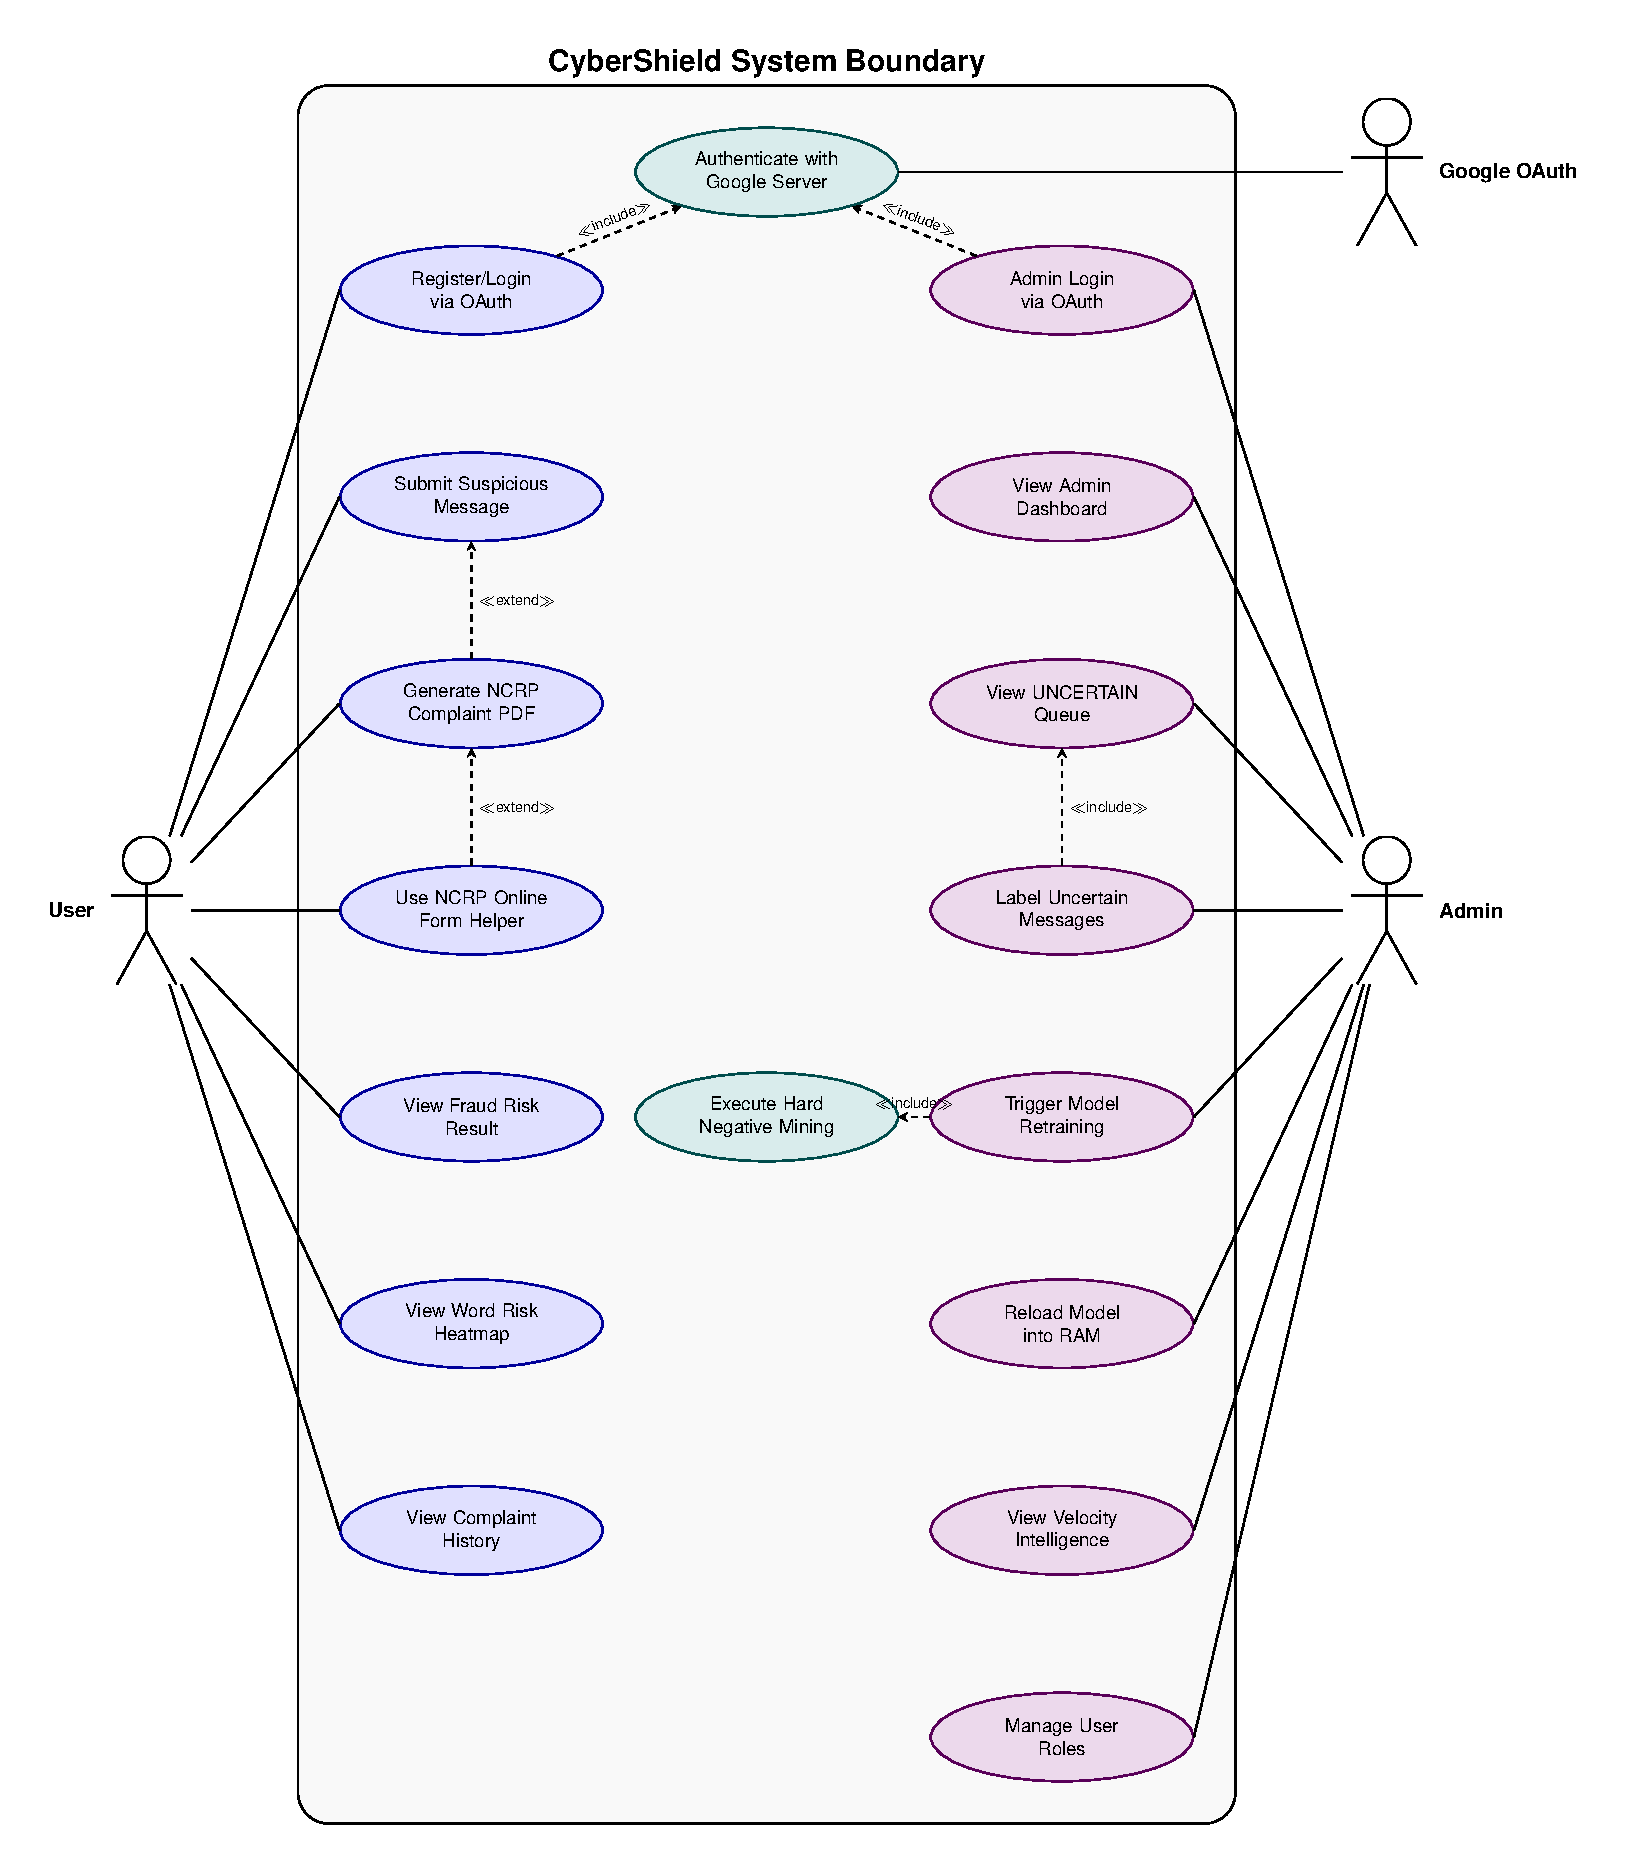
\includegraphics[width=0.85\textwidth]{figures/use_case_diagram.pdf}
    }
    \caption{Formal UML Use Case Diagram for CyberShield --- demonstrating the functional partition between public Citizen workflows and privileged Administrator controls, unified by a central Google OAuth authentication layer.}
    \label{fig:use_case}
\end{figure}

\section{Data Flow Diagrams}
A Data Flow Diagram (DFD) is a structured graphical tool that models the flow of information through a system, its transformations, storage, and interactions with external entities. Two levels are presented here.

\subsection{Level 0 DFD --- Context Diagram}
The Level 0 DFD, also known as the Context Diagram, represents the entire CyberShield system as a single process (Process 0) and defines its boundaries by identifying all external entities that interact with it, along with the high-level data flows between them.

\begin{figure}[H]
    \centering
    \resizebox{\textwidth}{!}{%
        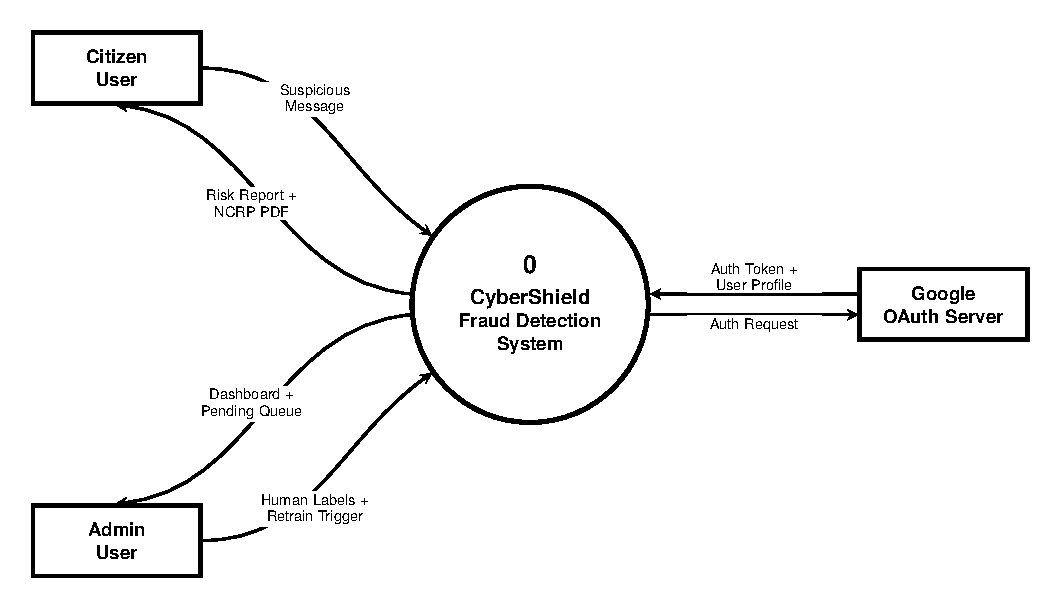
\includegraphics[width=0.85\textwidth]{figures/dfd_level0.pdf}
    }
    \caption{Level 0 DFD (Context Diagram) --- CyberShield system boundary with three external entities: Citizen User, Admin User, and Google OAuth Server, showing high-level input/output data flows.}
    \label{fig:dfd_level0}
\end{figure}

\subsection{Level 1 DFD --- Process Decomposition}
The Level 1 DFD decomposes Process 0 into five distinct functional sub-processes, exposes the four internal data stores, and traces every significant data flow between them and the external entities.

\begin{itemize}
    \item \textbf{P1 --- Authenticate User:} Mediates Google OAuth handshake for both citizen and admin sessions.
    \item \textbf{P2 --- Analyse Message:} Reads ML Models (D4), logs velocity indicators (D2), stores the complaint (D1), and queues uncertain results to D3.
    \item \textbf{P3 --- Generate Report:} Reads D1 to produce the risk heatmap and NCRP PDF returned to the citizen.
    \item \textbf{P4 --- Human Review:} Admin reads D3 (Pending Review DB) and writes human labels back.
    \item \textbf{P5 --- Retrain Model:} Triggered by admin; reads labeled data from D1 and D3, then updates D4 (ML model files).
\end{itemize}

\begin{figure}[H]
    \centering
    \resizebox{\textwidth}{!}{%
        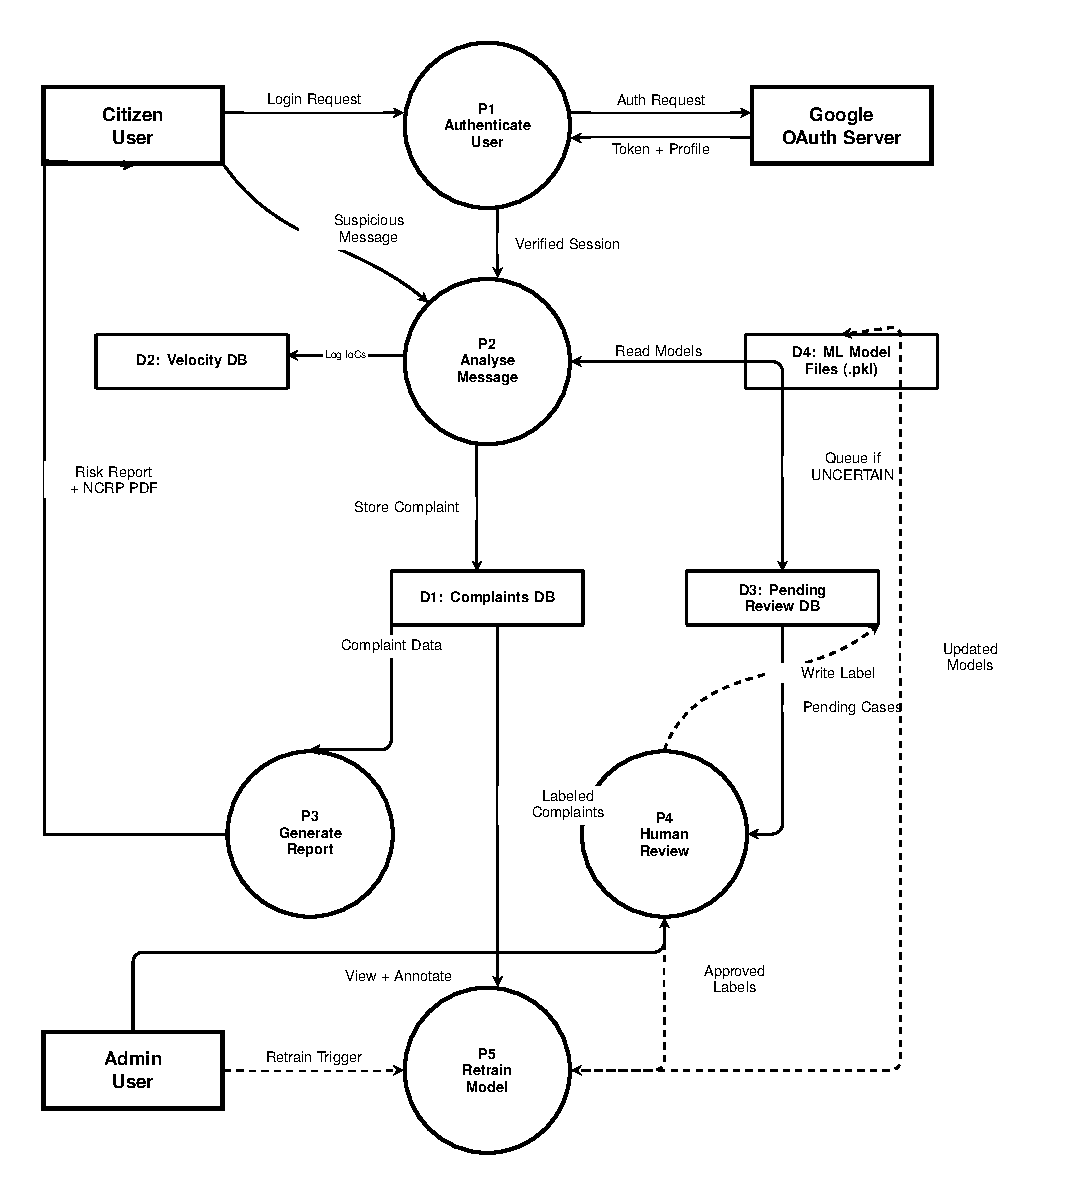
\includegraphics[width=0.85\textwidth]{figures/dfd_level1.pdf}
    }
    \caption{Level 1 DFD --- Decomposition of the CyberShield system into five processes (P1--P5) and four data stores (D1: Complaints, D2: Velocity, D3: Pending Review, D4: ML Models), with all inter-process and entity-to-process data flows.}
    \label{fig:dfd_level1}
\end{figure}

\section{Machine Learning Pipeline Design}
The core intelligence of CyberShield is designed around a three-stage mathematical pipeline: Preprocessing, Vectorization, and Ensemble Modeling.

\subsection{Preprocessing and Feature Extraction}
Raw text input is highly volatile. Before vectors can be mapped, the text undergoes:
\begin{enumerate}
    \item \textbf{Artifact Extraction:} The \texttt{preprocess()} function uses regular expressions to parse out and replace artifacts with semantic placeholder tokens rather than stripping them entirely. Specifically: URLs $\rightarrow$ \texttt{SUSPICIOUS\_URL}, Indian phone numbers (starting with 7/8/9) $\rightarrow$ \texttt{PHONE\_NUMBER}, rupee amounts $\rightarrow$ \texttt{MONEY\_AMOUNT}, USD amounts $\rightarrow$ \texttt{MONEY\_AMOUNT\_USD}, and 4--6 digit OTP patterns $\rightarrow$ \texttt{OTP\_NUMBER}. These tokens are retained as high-value fraud-signal features for the vectorizer.
    \item \textbf{Standardization:} Text is converted to lowercase, newline characters are stripped, and non-alphanumeric punctuation is removed to normalize the feature space.
\end{enumerate}

\begin{figure}[H]
    \centering
    \resizebox{\textwidth}{!}{
    \begin{tikzpicture}[
        node distance=1.5cm and 1.5cm,
        block/.style={rectangle, draw=black, thick, fill=white, text=black, text width=2.5cm, align=center, minimum height=1.2cm, rounded corners},
        arrow/.style={thick, ->, >=stealth, draw=black}
    ]
    \node[block] (raw) {Raw Text Input};
    \node[block, right=of raw] (regex) {RegEx Entity Extraction (URLs, Phones)};
    \node[block, below=of regex] (velocity) {Velocity Tracking DB};
    \node[block, right=of regex] (lower) {Lowercase \& Strip Punctuation};
    \node[block, right=of lower] (tfidf) {TF-IDF Vectorization ($25K$ features)};
    
    \node[block, right=of tfidf] (svm) {Support Vector Machine (SVM)};
    \node[block, above=0.5cm of svm] (lr) {Logistic Regression (LR)};
    \node[block, below=0.5cm of svm] (nb) {Naive Bayes (MNB)};
    
    \node[block, right=of svm] (predict) {Soft Voting Ensemble $P_{final}$};
    
    \draw[arrow] (raw) -- (regex);
    \draw[arrow] (regex) -- node[above=0.1cm, font=\footnotesize, align=center] {Sanitized\\String} (lower);
    \draw[arrow, dashed] (regex) -- node[right=0.1cm, font=\footnotesize] {Extracted IoCs} (velocity);
    \draw[arrow] (lower) -- (tfidf);
    
    \draw[arrow] (tfidf.east) -- ++(0.5,0) |- (lr.west);
    \draw[arrow] (tfidf.east) -- (svm.west);
    \draw[arrow] (tfidf.east) -- ++(0.5,0) |- (nb.west);
    
    \draw[arrow] (lr.east) -- ++(0.5,0) |- (predict.west);
    \draw[arrow] (svm.east) -- (predict.west);
    \draw[arrow] (nb.east) -- ++(0.5,0) |- (predict.west);
    \end{tikzpicture}
    }
    \caption{Level-1 Data Flow Diagram (DFD) of the ML Inference Loop --- illustrating the transformation of raw user input through artifact extraction, text sanitization, TF-IDF vectorization, and soft-voting ensemble scoring to produce the final probabilistic risk output $P_{final}$.}
    \label{fig:dfd}
\end{figure}

\subsection{TF-IDF Vectorization}
Term Frequency-Inverse Document Frequency (TF-IDF) represents words numerically \cite{salton1988term}. 
\begin{equation}
    \text{TF}(t, d) = \log(1 + f_{t,d})
\end{equation}
\begin{equation}
    \text{IDF}(t, D) = \log\left(\frac{N}{|\{d \in D : t \in d\}|}\right)
\end{equation}

\textbf{Notation Legend:}
\begin{itemize}
    \item $t$: A specific term (word or n-gram) in the vocabulary.
    \item $d$: A single document (message).
    \item $D$: The entire corpus of training documents.
    \item $N$: The total number of documents in the corpus.
    \item $f_{t,d}$: The raw frequency count of term $t$ in document $d$.
\end{itemize}

The implementation utilizes a Scikit-learn \texttt{FeatureUnion} \cite{pedregosa2011scikit} to combine two distinct vectorization strategies into a single $25,000$-feature space. The first component is a word n-gram vectorizer (\texttt{ngram\_range=(1,2)}, \texttt{max\_features=20000}, \texttt{sublinear\_tf=True}) with custom stopwords to capture semantic meaning. The second component is a character n-gram vectorizer (\texttt{analyzer='char\_wb'}, \texttt{ngram\_range=(3,5)}, \texttt{max\_features=5000}). This combined approach limits the vocabulary space due to RAM constraints (approximately 1GB) while the character n-grams explicitly provide robustness against adversarial obfuscation attacks (e.g., intentional misspellings).

\subsection{Soft-Voting Ensemble Logic}
An ensemble model prevents the weaknesses of any single algorithm from derailing the prediction \cite{dietterich2000ensemble}. The design utilizes:
\begin{itemize}
    \item \textbf{Logistic Regression (LR):} Provides highly calibrated probabilities \cite{cox1958regression}. Weight = 0.2
    \item \textbf{Support Vector Machine (SVM):} Deployed with a linear kernel, exceptionally proficient at drawing hyperplanes through high-dimensional text matrices \cite{cortes1995support}. Weight = 0.5
    \item \textbf{Multinomial Naive Bayes (MNB):} Calculates conditional probabilities based on Bayes' theorem, serving as a rapid baseline sanity check \cite{mccallum1998comparison}. Weight = 0.3
\end{itemize}

These weights are automatically tuned via a grid search over all valid weight triplets on the validation set during each retraining cycle, selecting the combination that maximizes macro-F1. The weights shown below represent the empirically optimal values from the current training run, not a manually fixed assignment. The final predictive probability is computed as shown in Equation \ref{eq:ensemble}:
\begin{equation}
\label{eq:ensemble}
    P_{final}(Fraud) = (0.2 \times P_{LR}) + (0.5 \times P_{SVM}) + (0.3 \times P_{NB})
\end{equation}
where $P_{final}(Fraud)$ is the ensembled probability score, and $P_{LR}$, $P_{SVM}$, and $P_{NB}$ are the individual fraud probabilities predicted by the Logistic Regression, Support Vector Machine, and Naive Bayes classifiers, respectively.

\section{Database Design}
CyberShield operates a lightweight SQLite database designed for rapid reads and simple structured queuing.
The schema logic comprises two primary operational architectures:

\subsection{User Identity and Authorization Schema}
The \texttt{users} table serves as the primary authentication and role-management ledger. Integrated with Google OAuth 2.0, this table tracks user identity and access privileges without storing sensitive passwords. Key fields include the user's primary email address, display name, and an administrative role flag. This table ensures that access to the Human-in-the-Loop (HITL) adjudication dashboard and retraining pipelines is strictly restricted to authorized administrators, preventing malicious actors from poisoning the active model.

\subsection{Citizen Submission and Routing Schema}
The v4 SQLAlchemy schema normalizes the database into four distinct tables: \texttt{users}, \texttt{complaints}, \texttt{velocity\_db}, and \texttt{pending\_review}. The \texttt{complaints} table acts as the historic lookup ledger for generated PDFs. The Human-in-the-Loop adjudication fields (\texttt{admin\_label} and \texttt{labeled\_by}) now reside exclusively in the \texttt{pending\_review} table. Figure \ref{fig:er_diagram} provides a visual representation of this normalized schema and its relationships. Table \ref{tab:complaints_schema} outlines the expanded fields of the \texttt{complaints} table.

\begin{table}[H]
    \centering
    \resizebox{\textwidth}{!}{
    \begin{tabular}{|l|l|l|l|}
    \hline
    \textbf{Column Name} & \textbf{Data Type} & \textbf{Constraint} & \textbf{Description} \\ \hline
    id & INTEGER & Primary Key, Auto-increment & Internal index tracker. \\ \hline
    user\_id & INTEGER & Foreign Key & Links complaint to a registered user. \\ \hline
    complaint\_id & VARCHAR(16) & Unique, Not Null & Hexadecimal UUID given to user. \\ \hline
    message & TEXT & Not Null & Raw string input payload. \\ \hline
    fraud\_probability & REAL & Range [0.0, 1.0] & Mathematical probability score. \\ \hline
    risk\_level & VARCHAR(12) & ENUM Constraint & FRAUD, SUSPICIOUS, UNCERTAIN, or LEGIT. \\ \hline
    fraud\_category & VARCHAR(50) & Nullable & Matched NCRP fraud category. \\ \hline
    ncrp\_code & VARCHAR(20) & Nullable & Generated NCRP Complaint Category Code. \\ \hline
    phones\_found & TEXT & Nullable & JSON array of extracted phone numbers. \\ \hline
    urls\_found & TEXT & Nullable & JSON array of extracted URLs. \\ \hline
    amounts\_found & TEXT & Nullable & JSON array of extracted monetary amounts. \\ \hline
    otps\_found & TEXT & Nullable & JSON array of extracted OTPs. \\ \hline
    keywords & TEXT & Nullable & JSON array of high-risk keywords. \\ \hline
    velocity\_alerts & TEXT & Nullable & JSON array of velocity tracking alerts. \\ \hline
    complainant\_name & VARCHAR(100) & Nullable & Name of the victim filing the report. \\ \hline
    complainant\_contact & VARCHAR(100) & Nullable & Contact information of the victim. \\ \hline
    sender & VARCHAR(100) & Nullable & Claimed sender of the malicious message. \\ \hline
    pdf\_path & VARCHAR(255) & Nullable & File path to the generated NCRP PDF. \\ \hline
    \end{tabular}
    }
    \caption{Entity-Relationship schema of the \texttt{complaints} table, illustrating the structural linkage between citizen submissions, extracted threat vectors, and assigned probabilistic risk scores.}
    \label{tab:complaints_schema}
\end{table}

\subsection{Velocity Tracking and Threat Intelligence Schema}
Velocity tracking in v4 is handled natively by the \texttt{velocity\_db} SQLAlchemy table rather than a flat JSON file, leveraging the ORM for concurrency management. The schema includes the following columns: \texttt{id} (Primary Key), \texttt{indicator\_type} (e.g., phone, url), \texttt{indicator\_value} (the artifact string), \texttt{count} (total hits), \texttt{complaint\_ids} (a JSON array of linked complaint IDs for traceability), \texttt{first\_seen} (timestamp), and \texttt{last\_seen} (timestamp). To ensure data integrity, a unique constraint is applied to the composite tuple \texttt{(indicator\_type, indicator\_value)}.

The velocity intelligence system assigns three formally defined threat tiers based on the cumulative occurrence count of each artifact across independent submissions:
\begin{itemize}
    \item \textbf{MED (count $= 1$):} An artifact encountered for the first time. MED represents a monitoring flag rather than an action trigger---the artifact is logged and tracked but does not yet constitute evidence of coordinated malicious activity.
    \item \textbf{HIGH (count $\geq 2$):} An artifact appearing across two or more independent victim submissions. A single malicious artifact seen across two independent reports indicates coordinated fraud activity rather than coincidence.
    \item \textbf{CRITICAL (count $\geq 4$):} A pragmatic operational threshold above which the artifact should be treated as an active campaign indicator warranting immediate administrative intervention.
\end{itemize}
These thresholds are heuristic and are recommended for empirical calibration against live deployment data in future iterations.

\subsection{Human-in-the-Loop Adjudication Queue Schema}
The \texttt{pending\_review} table is the operational core of the Human-in-the-Loop calibration system. It acts as an isolation queue for all messages classified as UNCERTAIN ($0.30 \leq P(Fraud) < 0.70$). Rather than polluting the historical \texttt{complaints} ledger with unverified machine annotations, ambiguous cases are safely parked here. The schema includes fields for the raw message, the initial model probabilities, and critical adjudication fields: \texttt{admin\_label} (the final human verdict) and \texttt{labeled\_by} (tracking which administrator made the decision for audit purposes). Once adjudicated, these records are harvested by the \texttt{pipefinal.py} script for Hard Negative Mining.

\begin{figure}[H]
    \centering
    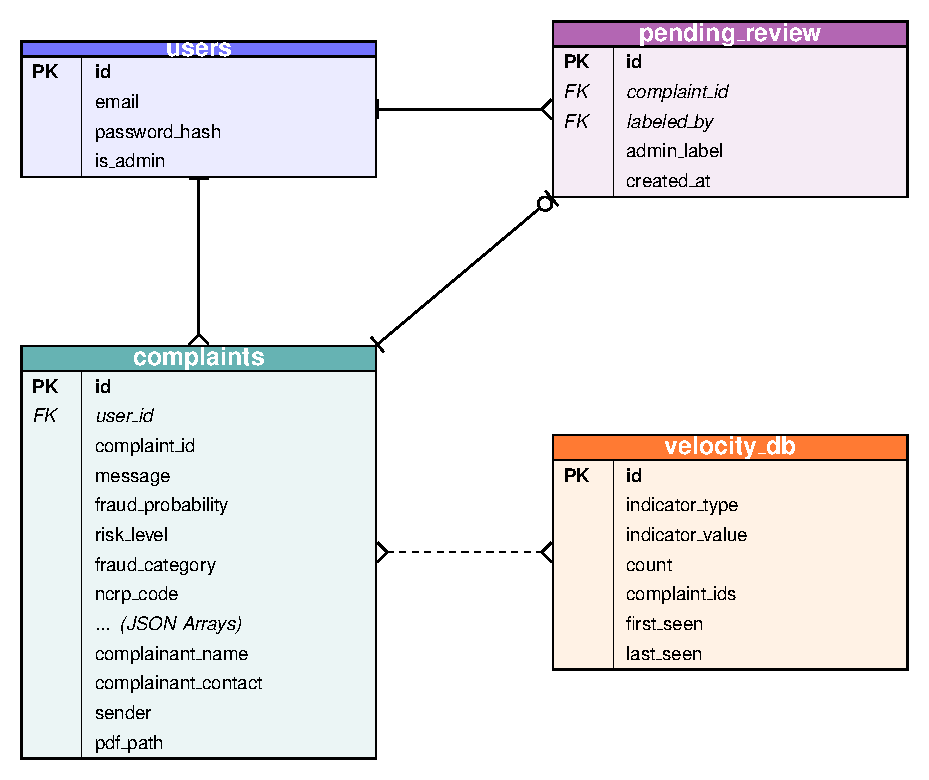
\includegraphics[width=0.85\textwidth]{figures/er_diagram.pdf}
    \caption{Entity-Relationship diagram of the v4 CyberShield database schema, outlining the linkages between users, complaints, velocity tracking, and manual annotations.}
    \label{fig:er_diagram}
\end{figure}

\section{Human-in-the-Loop (HITL) Design Workflow}
Traditional systems are fully autonomous. CyberShield is designed as a semi-autonomous calibration loop that acknowledges uncertainty \cite{holzinger2016interactive}. The workflow proceeds as follows:
\begin{enumerate}
    \item \textbf{Inference:} User submits a message. $P_{final}$ calculates to $0.42$.
    \item \textbf{Routing:} The threshold logic catches $0.42$ in the $0.30 - 0.70$ boundary. Risk is set to UNCERTAIN.
    \item \textbf{Queuing:} The record is saved in the \texttt{complaints} table with \texttt{admin\_label = NULL}.
    \item \textbf{Adjudication:} An Admin logs into \texttt{/admin}. The dashboard queries all records where \texttt{admin\_label} is NULL. The admin reads the context and officially tags it as `fraud`.
    \item \textbf{Mining:} When the admin triggers \texttt{Retrain Model}, the \texttt{pipefinal.py} script awakens. It queries the DB for all non-NULL \texttt{admin\_label} entries.
    \item \textbf{Training Integration:} These newly labeled samples are strictly injected into the Training array. The model undergoes vectorization and applies Hard Negative Mining algorithms, significantly adjusting the decision boundary to guarantee that similar linguistic patterns will permanently register above $0.90$ probability in the future.
    \item \textbf{Model Activation:} Upon successful completion of \texttt{pipefinal.py}, the new \texttt{final\_models.pkl} and \texttt{final\_vectorizer.pkl} are written to disk. The admin clicks the Reload Model button, which triggers the \texttt{/admin/reload-model} route, hot-loading the new pickle files into RAM without requiring a server restart.
\end{enumerate}

\begin{figure}[H]
    \centering
    \resizebox{\textwidth}{!}{
    \begin{tikzpicture}[
        node distance=1.5cm and 2cm,
        decision/.style={diamond, draw, thick, text width=2.8cm, align=center, inner sep=0pt, fill=gray!12},
        block/.style={rectangle, draw, thick, text width=3.8cm, align=center, rounded corners, minimum height=1.2cm, fill=white},
        term/.style={rectangle, draw, thick, text width=3.8cm, align=center, rounded corners=15pt, minimum height=1.2cm},
        arrow/.style={thick, ->, >=stealth}
    ]
    
    \node[block, fill=gray!10] (input) {\textbf{Receive $P_{final}$}\\From Soft-Voting Ensemble};
    \node[decision, below=of input] (d1) {\textbf{FRAUD?}\\$P \geq 0.90$};
    \node[term, right=of d1, fill=red!30, draw=red!70!black] (fraud) {\textbf{Mark as FRAUD}\\Auto-Adjudicated\\Generate NCRP PDF};
    
    \node[decision, below=of d1] (d2) {\textbf{SUSPICIOUS?}\\$P \geq 0.70$};
    \node[term, right=of d2, fill=orange!35, draw=orange!80!black] (susp) {\textbf{Mark SUSPICIOUS}\\Dashboard Alert\\No NCRP Trigger};
    
    \node[decision, below=of d2] (d3) {\textbf{UNCERTAIN?}\\$P \geq 0.30$};
    \node[block, right=of d3, fill=yellow!40, draw=yellow!80!black] (unc) {\textbf{Mark UNCERTAIN}\\Queue for HITL review};
    \node[block, right=of unc, fill=yellow!20, draw=yellow!60!black] (admin) {\textbf{Admin Review}\\Manual Annotation};
    \node[term, right=of admin, fill=yellow!25, draw=orange!60!black] (retrain) {\textbf{Trigger Retrain}\\Hard Negative Mining};
    
    \node[term, below=of d3, fill=green!25, draw=green!60!black] (legit) {\textbf{Mark LEGIT}\\Normal Processing};
    
    \draw[arrow] (input) -- (d1);
    \draw[arrow] (d1) -- node[above] {Yes} (fraud);
    \draw[arrow] (d1) -- node[right] {No} (d2);
    
    \draw[arrow] (d2) -- node[above] {Yes} (susp);
    \draw[arrow] (d2) -- node[right] {No} (d3);
    
    \draw[arrow] (d3) -- node[above] {Yes} (unc);
    \draw[arrow] (d3) -- node[right] {No} (legit);
    
    \draw[arrow] (unc) -- (admin);
    \draw[arrow] (admin) -- (retrain);
    \end{tikzpicture}
    }
    \caption{Human-in-the-Loop Threshold Decision Flowchart --- showing the four-tier probabilistic routing logic. Messages with $P_{final} \geq 0.90$ are auto-adjudicated as FRAUD; those between $0.70\text{--}0.90$ as SUSPICIOUS; those between $0.30\text{--}0.70$ are queued as UNCERTAIN for human review and subsequent Hard Negative Mining retraining; those below $0.30$ are marked LEGIT.}
    \label{fig:hitl}
\end{figure}

\section{Serialized Artifact Design}
The intelligence of CyberShield does not persist within standard relational tables but is serialized into highly compressed binary files utilizing the \texttt{pickle} and \texttt{joblib} modules. The architecture mandates three distinct serialized artifacts:
\begin{itemize}
    \item \texttt{split\_indices.pkl}: Stores frozen integer index arrays for the Train, Validation, and Test splits. This artifact guarantees data continuity and mathematical reproducibility across infinite retraining cycles.
    \item \texttt{final\_vectorizer.pkl}: Stores the fitted \texttt{TfidfVectorizer} object comprising the $25,000$-feature vocabulary, fitted exclusively on the training array subset.
    \item \texttt{final\_models.pkl}: Stores the three fitted classifier objects (LR, SVM, NB) along with their calibration wrappers to ensure accurate probabilistic outputs.
\end{itemize}
These files are aggressively written to the disk subsystem by \texttt{pipefinal.py} post-training. During the boot sequence, the Flask application (\texttt{app.py}) ingests these files entirely into RAM. Therefore, overwriting these files is the explicit mechanism by which the retraining module updates the live inference system without requiring database migrations.

\section{API Route Design}
The system routes interact via standard REST protocols. Table \ref{tab:api_routes} defines the primary endpoints driving the CyberShield web architecture.

\begin{table}[H]
    \centering
    \resizebox{\textwidth}{!}{
    \begin{tabular}{|l|l|l|l|}
    \hline
    \textbf{Route} & \textbf{Method} & \textbf{Auth Required} & \textbf{Purpose} \\ \hline
    \texttt{/} & GET & No & Serves the citizen-facing home interface. \\ \hline
    \texttt{/analyze} & POST & Yes (Google OAuth) & Accepts raw text, returns probabilistic risk and extracted artifacts. \\ \hline
    \texttt{/generate-pdf} & POST & Yes (Google OAuth) & Generates NCRP-compliant PDF; \texttt{complaint\_id} must belong to the requesting user. \\ \hline
    \texttt{/download-complaint/<id>} & GET & Yes (Google OAuth) & Downloads the PDF; validates \texttt{complaint\_id} ownership before serving. \\ \hline
    \texttt{/ncrp-helper/<id>} & GET & No & Serves the helper interface for manual NCRP filing. \\ \hline
    \texttt{/history} & GET & Yes & Displays the complaint history for the logged-in user. \\ \hline
    \texttt{/admin} & GET & OAuth (Whitelisted Email) & Serves the admin dashboard showing pending UNCERTAIN queue. \\ \hline
    \texttt{/admin/label} & POST & OAuth (Whitelisted Email) & Writes human annotation (fraud/legit) to a complaint record. \\ \hline
    \texttt{/admin/retrain} & POST & OAuth (Whitelisted Email) & Triggers asynchronous \texttt{pipefinal.py} subprocess to retrain the model. \\ \hline
    \texttt{/admin/reload-model} & POST & Admin & Hot-loads newly trained models into RAM. \\ \hline
    \texttt{/admin/retrain-status} & GET & Admin & Polls the status of the background retraining task. \\ \hline
    \texttt{/admin/velocity-db} & GET & Admin & Serves the Velocity Intelligence threat dashboard. \\ \hline
    \texttt{/admin/users} & GET & Admin & Serves the user management panel. \\ \hline
    \texttt{/admin/users/<id>/toggle-admin} & POST & Admin & Promotes or demotes a user's admin privileges. \\ \hline
    \end{tabular}
    }
    \caption{Overview of defined API routes, detailing HTTP methods, endpoint URIs, and their respective functional purposes within the CyberShield architecture.}
    \label{tab:api_routes}
\end{table}

\section{Failure Mode and Error Handling Design}
To guarantee a resilient production deployment, the architecture proactively defends against the following failure permutations:
\begin{enumerate}
    \item \textbf{Missing Artifacts:} If \texttt{final\_models.pkl} or \texttt{final\_vectorizer.pkl} are missing on server boot, Flask will purposefully raise a fatal startup exception with a descriptive error message rather than failing silently at inference time.
    \item \textbf{Database Concurrency:} SQLAlchemy's connection pool manages concurrent database access, providing thread-safe read/write operations across simultaneous requests without requiring manual WAL configuration.
    \item \textbf{Retrain Subprocess Crash:} If the \texttt{pipefinal.py} retraining subprocess crashes midway (e.g., due to an Out-of-Memory error), the existing pickle files are left completely untouched. The script is programmed to only overwrite the local artifacts upon a fully successful completion routine, meaning partial failures do not corrupt the live model.
    \item \textbf{Conversational False Positives:} Short benign messages (e.g., ``Hi'', ``Thanks'') can cross the 0.30 UNCERTAIN threshold and pollute the admin queue. A deterministic colloquial override forces $P(\text{Fraud}) = 0.05$ for conversational regex matches when the raw ensemble probability is below 0.50, while intentionally leaving predictions above 0.50 unsuppressed to avoid masking genuinely malicious openers.
\end{enumerate}

\section{End-to-End System Pipeline Flow}
Figure~\ref{fig:pipeline_flow} maps the complete data processing pipeline across ten stages and five functional swimlanes: Citizen, Flask Controller, ML Intelligence Layer, SQLite Database, and Administrator. Stages~9 and~10 illustrate the isolated HITL calibration and Hard Negative Mining feedback loop, enabling the model to adapt over time without server restarts.

\begin{figure}[H]
    \centering
    \resizebox{\textwidth}{!}{
        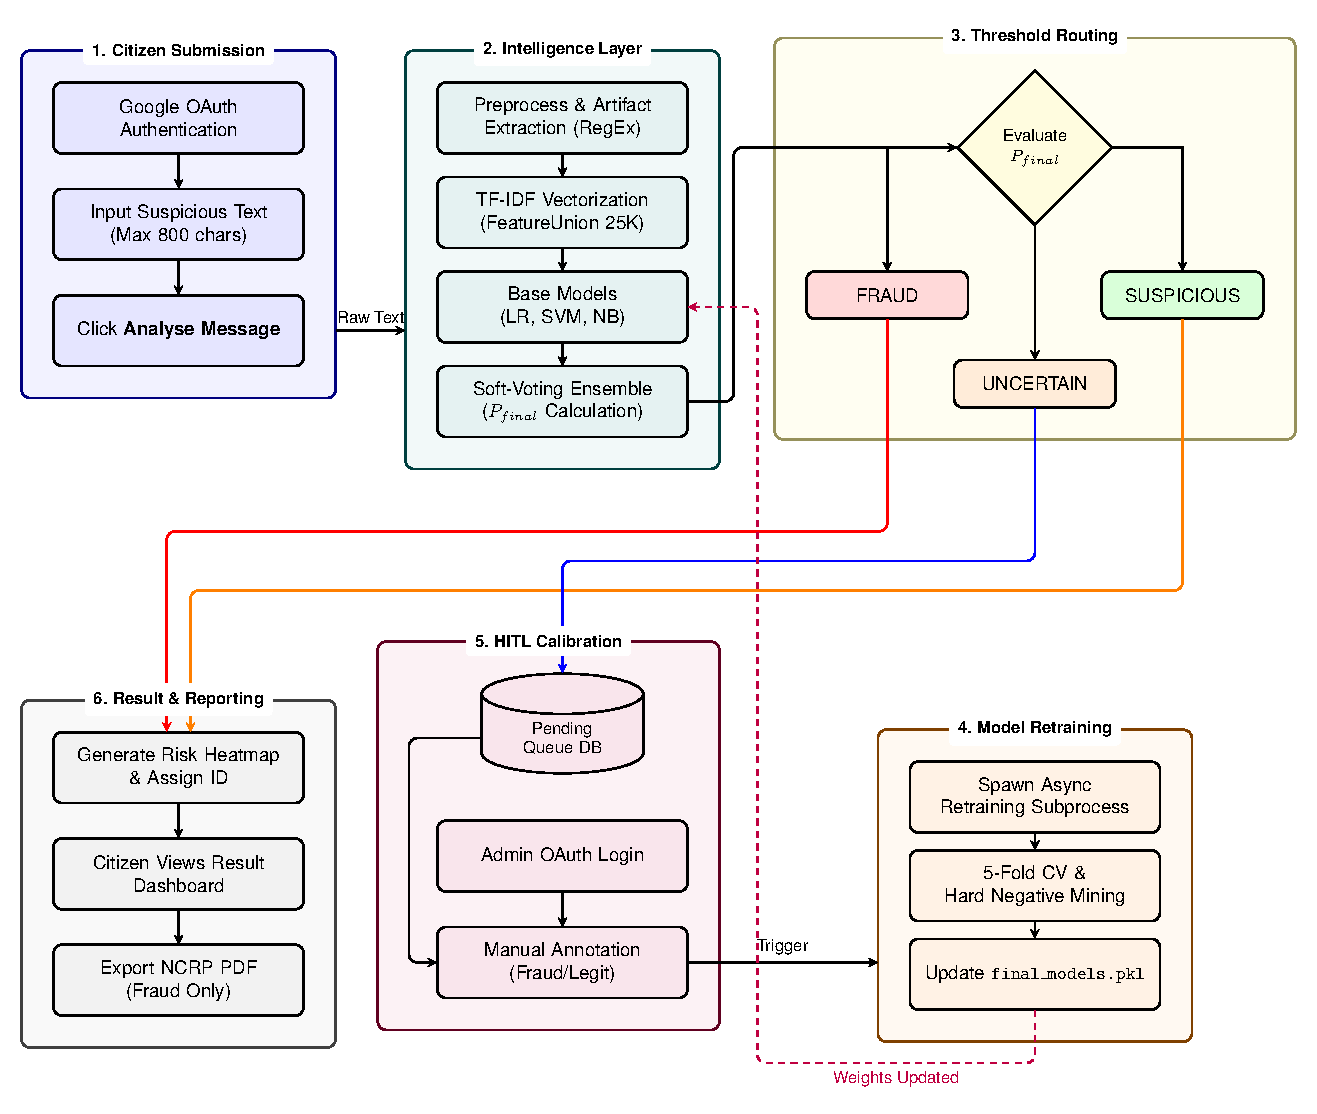
\includegraphics[width=0.85\textwidth]{figures/pipeline_flow.pdf}
    }
    \caption{End-to-End System Pipeline Flow Diagram mapping the 10-stage lifecycle across all architectural layers, including the offline asynchronous retraining loop.}
    \label{fig:pipeline_flow}
\end{figure}
